\begin{figure}[htbp]
\centering
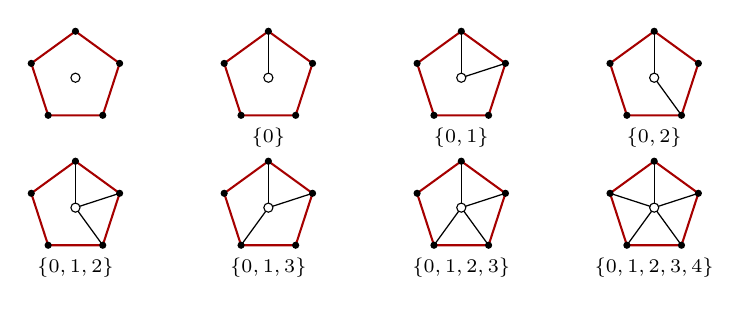
\begin{tikzpicture}[font=\scriptsize,
sc marked/.style={draw=red!65!black,line width=.75pt},
sc unmarked/.style={draw=blue!65!black,line width=.68pt,dash pattern=on 1.5pt off 1.35pt}]
\begin{scope}[shift={(-3.675,0)}]
\coordinate (c0) at (90:.59);
\coordinate (c1) at (18:.59);
\coordinate (c2) at (-54:.59);
\coordinate (c3) at (-126:.59);
\coordinate (c4) at (-198:.59);
\draw[sc marked] (c0)--(c1)--(c2)--(c3)--(c4)--cycle;
\fill (c0) circle[radius=1.3pt];
\fill (c1) circle[radius=1.3pt];
\fill (c2) circle[radius=1.3pt];
\fill (c3) circle[radius=1.3pt];
\fill (c4) circle[radius=1.3pt];
\draw[fill=white] (0,0) circle[radius=1.65pt];
\node at (0,-.76) {\(\varnothing\)};
\end{scope}
\begin{scope}[shift={(-1.225,0)}]
\coordinate (c0) at (90:.59);
\coordinate (c1) at (18:.59);
\coordinate (c2) at (-54:.59);
\coordinate (c3) at (-126:.59);
\coordinate (c4) at (-198:.59);
\draw[sc marked] (c0)--(c1)--(c2)--(c3)--(c4)--cycle;
\draw[black,line width=.45pt] (0,0)--(c0);
\fill (c0) circle[radius=1.3pt];
\fill (c1) circle[radius=1.3pt];
\fill (c2) circle[radius=1.3pt];
\fill (c3) circle[radius=1.3pt];
\fill (c4) circle[radius=1.3pt];
\draw[fill=white] (0,0) circle[radius=1.65pt];
\node at (0,-.76) {\(\{0\}\)};
\end{scope}
\begin{scope}[shift={(1.225,0)}]
\coordinate (c0) at (90:.59);
\coordinate (c1) at (18:.59);
\coordinate (c2) at (-54:.59);
\coordinate (c3) at (-126:.59);
\coordinate (c4) at (-198:.59);
\draw[sc marked] (c0)--(c1)--(c2)--(c3)--(c4)--cycle;
\draw[black,line width=.45pt] (0,0)--(c0);
\draw[black,line width=.45pt] (0,0)--(c1);
\fill (c0) circle[radius=1.3pt];
\fill (c1) circle[radius=1.3pt];
\fill (c2) circle[radius=1.3pt];
\fill (c3) circle[radius=1.3pt];
\fill (c4) circle[radius=1.3pt];
\draw[fill=white] (0,0) circle[radius=1.65pt];
\node at (0,-.76) {\(\{0,1\}\)};
\end{scope}
\begin{scope}[shift={(3.675,0)}]
\coordinate (c0) at (90:.59);
\coordinate (c1) at (18:.59);
\coordinate (c2) at (-54:.59);
\coordinate (c3) at (-126:.59);
\coordinate (c4) at (-198:.59);
\draw[sc marked] (c0)--(c1)--(c2)--(c3)--(c4)--cycle;
\draw[black,line width=.45pt] (0,0)--(c0);
\draw[black,line width=.45pt] (0,0)--(c2);
\fill (c0) circle[radius=1.3pt];
\fill (c1) circle[radius=1.3pt];
\fill (c2) circle[radius=1.3pt];
\fill (c3) circle[radius=1.3pt];
\fill (c4) circle[radius=1.3pt];
\draw[fill=white] (0,0) circle[radius=1.65pt];
\node at (0,-.76) {\(\{0,2\}\)};
\end{scope}
\begin{scope}[shift={(-3.675,-1.65)}]
\coordinate (c0) at (90:.59);
\coordinate (c1) at (18:.59);
\coordinate (c2) at (-54:.59);
\coordinate (c3) at (-126:.59);
\coordinate (c4) at (-198:.59);
\draw[sc marked] (c0)--(c1)--(c2)--(c3)--(c4)--cycle;
\draw[black,line width=.45pt] (0,0)--(c0);
\draw[black,line width=.45pt] (0,0)--(c1);
\draw[black,line width=.45pt] (0,0)--(c2);
\fill (c0) circle[radius=1.3pt];
\fill (c1) circle[radius=1.3pt];
\fill (c2) circle[radius=1.3pt];
\fill (c3) circle[radius=1.3pt];
\fill (c4) circle[radius=1.3pt];
\draw[fill=white] (0,0) circle[radius=1.65pt];
\node at (0,-.76) {\(\{0,1,2\}\)};
\end{scope}
\begin{scope}[shift={(-1.225,-1.65)}]
\coordinate (c0) at (90:.59);
\coordinate (c1) at (18:.59);
\coordinate (c2) at (-54:.59);
\coordinate (c3) at (-126:.59);
\coordinate (c4) at (-198:.59);
\draw[sc marked] (c0)--(c1)--(c2)--(c3)--(c4)--cycle;
\draw[black,line width=.45pt] (0,0)--(c0);
\draw[black,line width=.45pt] (0,0)--(c1);
\draw[black,line width=.45pt] (0,0)--(c3);
\fill (c0) circle[radius=1.3pt];
\fill (c1) circle[radius=1.3pt];
\fill (c2) circle[radius=1.3pt];
\fill (c3) circle[radius=1.3pt];
\fill (c4) circle[radius=1.3pt];
\draw[fill=white] (0,0) circle[radius=1.65pt];
\node at (0,-.76) {\(\{0,1,3\}\)};
\end{scope}
\begin{scope}[shift={(1.225,-1.65)}]
\coordinate (c0) at (90:.59);
\coordinate (c1) at (18:.59);
\coordinate (c2) at (-54:.59);
\coordinate (c3) at (-126:.59);
\coordinate (c4) at (-198:.59);
\draw[sc marked] (c0)--(c1)--(c2)--(c3)--(c4)--cycle;
\draw[black,line width=.45pt] (0,0)--(c0);
\draw[black,line width=.45pt] (0,0)--(c1);
\draw[black,line width=.45pt] (0,0)--(c2);
\draw[black,line width=.45pt] (0,0)--(c3);
\fill (c0) circle[radius=1.3pt];
\fill (c1) circle[radius=1.3pt];
\fill (c2) circle[radius=1.3pt];
\fill (c3) circle[radius=1.3pt];
\fill (c4) circle[radius=1.3pt];
\draw[fill=white] (0,0) circle[radius=1.65pt];
\node at (0,-.76) {\(\{0,1,2,3\}\)};
\end{scope}
\begin{scope}[shift={(3.675,-1.65)}]
\coordinate (c0) at (90:.59);
\coordinate (c1) at (18:.59);
\coordinate (c2) at (-54:.59);
\coordinate (c3) at (-126:.59);
\coordinate (c4) at (-198:.59);
\draw[sc marked] (c0)--(c1)--(c2)--(c3)--(c4)--cycle;
\draw[black,line width=.45pt] (0,0)--(c0);
\draw[black,line width=.45pt] (0,0)--(c1);
\draw[black,line width=.45pt] (0,0)--(c2);
\draw[black,line width=.45pt] (0,0)--(c3);
\draw[black,line width=.45pt] (0,0)--(c4);
\fill (c0) circle[radius=1.3pt];
\fill (c1) circle[radius=1.3pt];
\fill (c2) circle[radius=1.3pt];
\fill (c3) circle[radius=1.3pt];
\fill (c4) circle[radius=1.3pt];
\draw[fill=white] (0,0) circle[radius=1.65pt];
\node at (0,-.76) {\(\{0,1,2,3,4\}\)};
\end{scope}
\end{tikzpicture}
\caption{The eight possible neighborhoods of one exterior vertex on the cycle, up to rotation and reflection. The open vertex is $x$. The cycle vertices are indexed clockwise from the top. A spoke indicates adjacency to $x$ and can be marked or unmarked.}
\label{fig:finite-simple-signatures}
\end{figure}
